%In this section we document the expected separation between 
%the SM Higgs and $2_\text{min}^+$ graviton hypotheses for \intlumiEightTeV at 8 TeV.  

To calculate the expected separation between the SM Higgs and other 
exotic resonances, we use the same number of events for the exotic resonance
after the full selections as in the SM Higgs case. 

Figure~\ref{fig:expsep} shows the distributions of 
$q=-2\text{ln}({\cal L}_{2_\text{min}^+}/{\cal L}_{\text{0}^+})$
with generated samples of background and signal of the SM Higgs and 
$2_\text{min}^+$ Graviton at 125 GeV. 
The yields used in the generation of the pseudo-experiments are those 
expected with \intlumiEightTeV at 8 TeV. 
%SM $0^+$ and minimal couplings spin 2 $2_\text{min}^+$, for $m_H=$125 GeV. 
%The expected distributions are generated with the same number of events 
%after the full event selections. 
The mean of the expected SM $0^+$ distribution is 1.5 standard deviations 
in the tail of the $2_\text{min}^+$ distribution, while 
the mean of the expected $2_\text{min}^+$ distribution is 1.2 standard deviations 
in the tail of the $0^+$ distribution. 
The average separation between the two hypothesis is about $1.3\sigma$. 
The signal to background significance expected on average 
for the SM Higgs hypothesis is $3.3\sigma$, while for the spin 2 graviton $2_\text{min}^+$ 
model it is around $2.6\sigma$. 
%Scaling purely by luminosity, 
The expected average separation between the SM Higgs and $2_\text{min}^+$ 
hypotheses is about $1.7\sigma$ for 30~$\ifb$ scaling purely by luminosity. 


%%%%%%%%%%%%%%%%%%%%%%%%%%%%%%%%%%%%%%%%%%%%%
\begin{figure}[!hbtp]
\centering
\label{subfig:res}
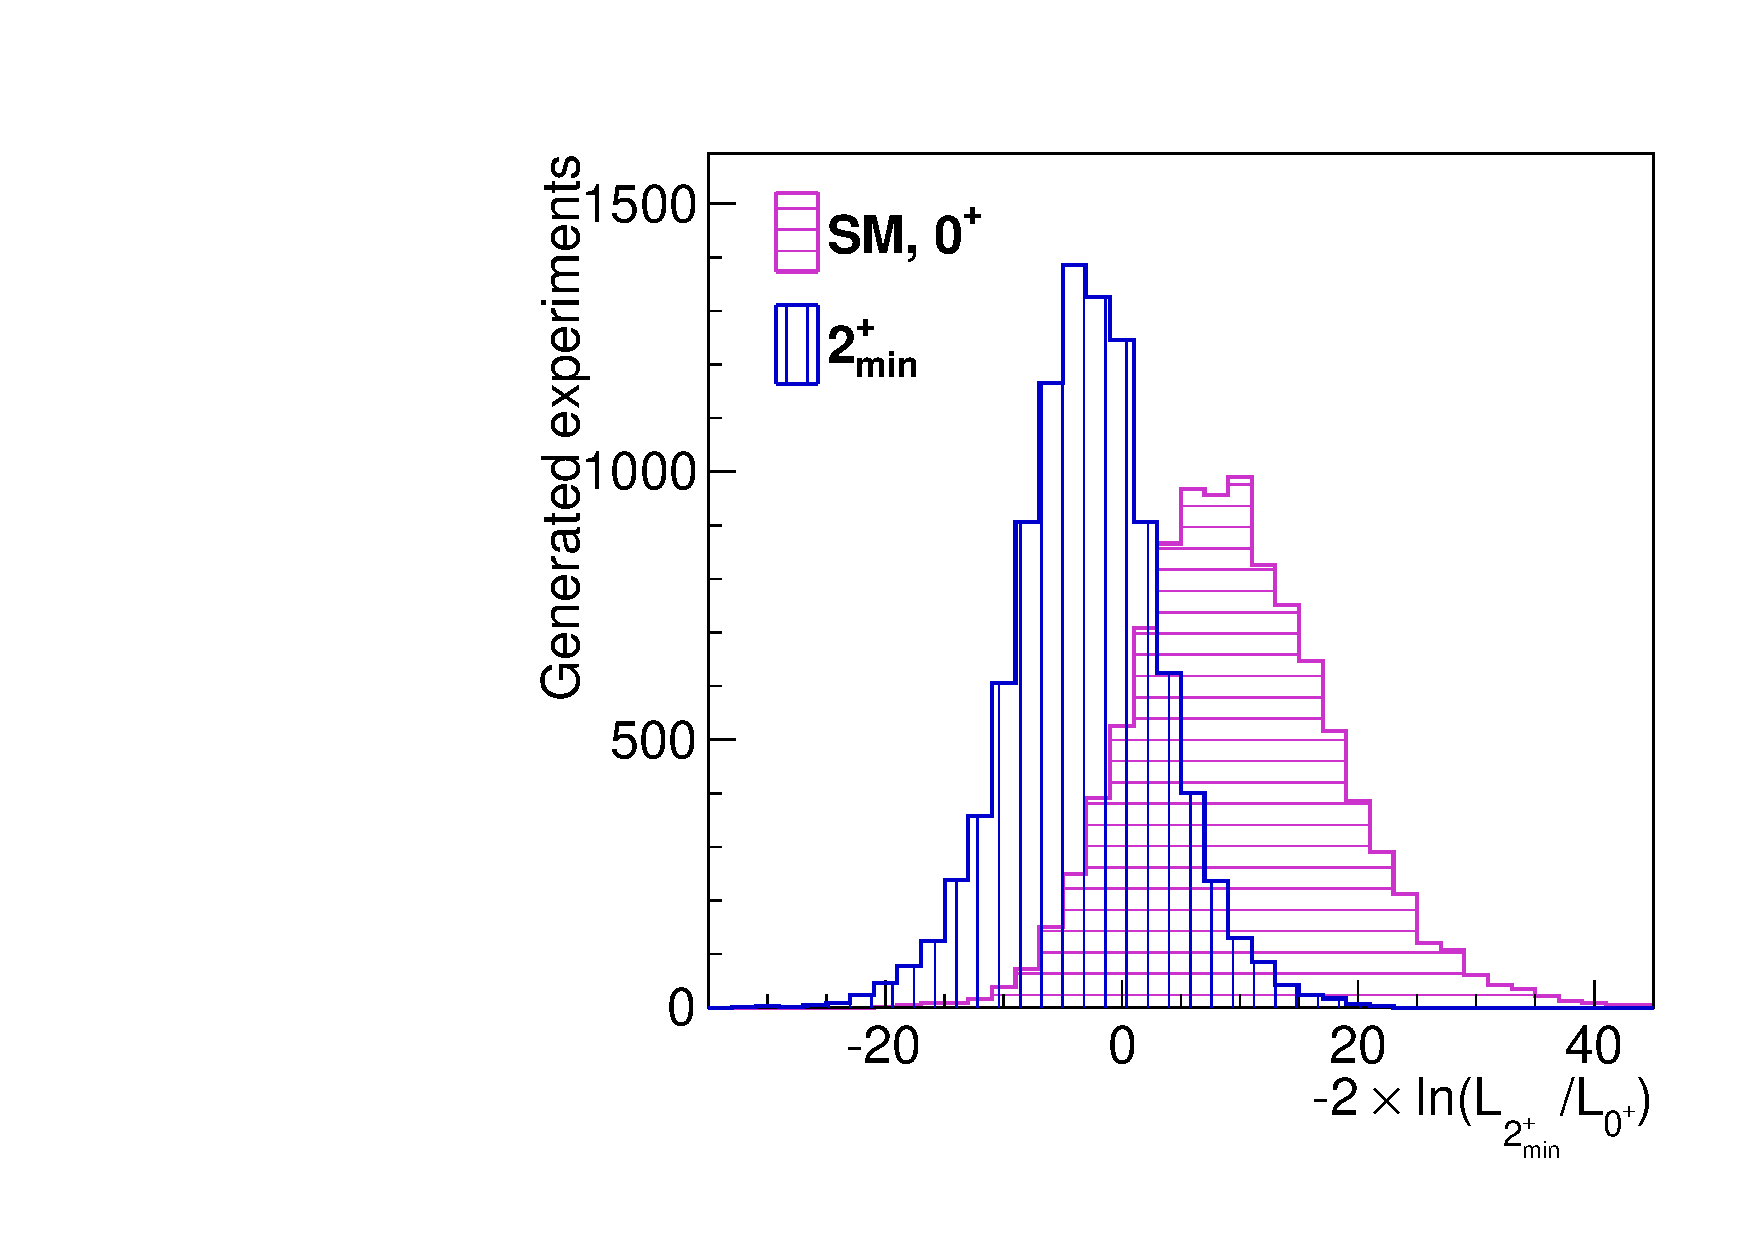
\includegraphics[width=.7\textwidth]{figures/hypo_separation.pdf}
\caption{Distributions of 
$q=-2\text{ln}({\cal L}_{2_\text{min}^+}/{\cal L}_{\text{0}^+})$ 
of 50K pseudo-experiments according to two signal types, $0^+$ (horizontally hatched histogram) 
and $2_\text{min}^+$ (vertically hatched histogram) at $m_H=$125 GeV. 
The yields used in the generation of the pseudo-experiments are those 
expected with \intlumiEightTeV at 8 TeV. 
}
\label{fig:expsep}
\end{figure}
%%%%%%%%%%%%%%%%%%%%%%%%%%%%%%%%%%%%%%%%%%%%%

